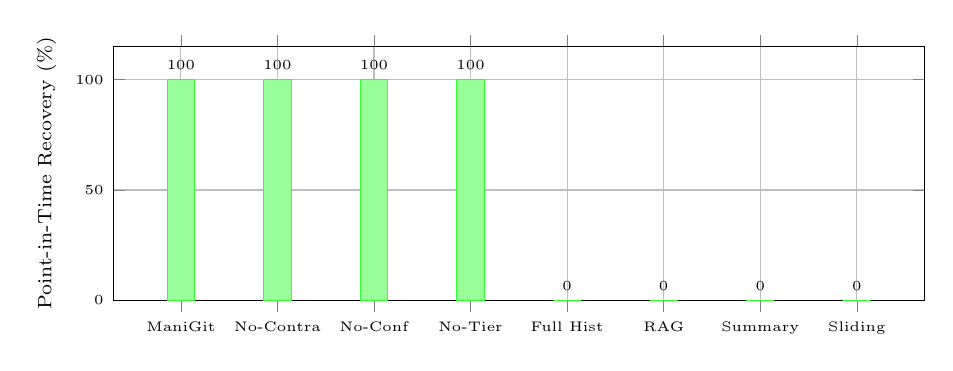
\begin{tikzpicture}
\begin{axis}[
    ybar,
    width=0.98\columnwidth, height=4.8cm,
    symbolic x coords={ManiGit, No-Contra, No-Conf, No-Tier, Full Hist, RAG, Summary, Sliding},
    xtick=data,
    ylabel={Point-in-Time Recovery (\%)},
    ymin=0, ymax=115,
    nodes near coords,
    nodes near coords style={font=\tiny},
    grid=both,
    tick label style={font=\tiny},
    label style={font=\scriptsize}
]
\addplot[fill=green!40, draw=green!80] coordinates {
    (ManiGit, 100) (No-Contra, 100) (No-Conf, 100) (No-Tier, 100) (Full Hist, 0) (RAG, 0) (Summary, 0) (Sliding, 0)
};
\end{axis}
\end{tikzpicture}
